% !TEX root = main.tex
\section{Coil Analysis}
\label{sec:CoilAnalyssis}
Now knowing that we have an acceptable noise value of less than \SI{10}{\mu \volt}, we can analyse the coil.
In order to do so we explain the general approach of NMR signals first.
To measure a NMR signal a pulse and collect measurement has to be done.
Therefore the B$_1$ coil (transmit and collect coil) has to apply a pulse.
This pulse changes the spins direction out of its thermal equilibrium (along z-axes, due to the earths magnetic field B$_e$) into a direction with a component in the transversal plain.
Therefore the B$_1$ coil collects a signal because it is aligned orthogonal to B$_e$.
The transmit and collect procedure is based on \textsc{Faraday}'s law of induction.
Figure \ref{fig: PulsandcollectValesignal} exemplary shows such a pulse and collect signal by the B$_1$ coil.
Every following measurement in this report is based on the procedure of pulse and collect.

\begin{figure}[H]
    \centering
    % GNUPLOT: LaTeX picture with Postscript
\begingroup
  % Encoding inside the plot.  In the header of your document, this encoding
  % should to defined, e.g., by using
  % \usepackage[cp1252,<other encodings>]{inputenc}
  \inputencoding{cp1252}%
  \makeatletter
  \providecommand\color[2][]{%
    \GenericError{(gnuplot) \space\space\space\@spaces}{%
      Package color not loaded in conjunction with
      terminal option `colourtext'%
    }{See the gnuplot documentation for explanation.%
    }{Either use 'blacktext' in gnuplot or load the package
      color.sty in LaTeX.}%
    \renewcommand\color[2][]{}%
  }%
  \providecommand\includegraphics[2][]{%
    \GenericError{(gnuplot) \space\space\space\@spaces}{%
      Package graphicx or graphics not loaded%
    }{See the gnuplot documentation for explanation.%
    }{The gnuplot epslatex terminal needs graphicx.sty or graphics.sty.}%
    \renewcommand\includegraphics[2][]{}%
  }%
  \providecommand\rotatebox[2]{#2}%
  \@ifundefined{ifGPcolor}{%
    \newif\ifGPcolor
    \GPcolorfalse
  }{}%
  \@ifundefined{ifGPblacktext}{%
    \newif\ifGPblacktext
    \GPblacktexttrue
  }{}%
  % define a \g@addto@macro without @ in the name:
  \let\gplgaddtomacro\g@addto@macro
  % define empty templates for all commands taking text:
  \gdef\gplbacktext{}%
  \gdef\gplfronttext{}%
  \makeatother
  \ifGPblacktext
    % no textcolor at all
    \def\colorrgb#1{}%
    \def\colorgray#1{}%
  \else
    % gray or color?
    \ifGPcolor
      \def\colorrgb#1{\color[rgb]{#1}}%
      \def\colorgray#1{\color[gray]{#1}}%
      \expandafter\def\csname LTw\endcsname{\color{white}}%
      \expandafter\def\csname LTb\endcsname{\color{black}}%
      \expandafter\def\csname LTa\endcsname{\color{black}}%
      \expandafter\def\csname LT0\endcsname{\color[rgb]{1,0,0}}%
      \expandafter\def\csname LT1\endcsname{\color[rgb]{0,1,0}}%
      \expandafter\def\csname LT2\endcsname{\color[rgb]{0,0,1}}%
      \expandafter\def\csname LT3\endcsname{\color[rgb]{1,0,1}}%
      \expandafter\def\csname LT4\endcsname{\color[rgb]{0,1,1}}%
      \expandafter\def\csname LT5\endcsname{\color[rgb]{1,1,0}}%
      \expandafter\def\csname LT6\endcsname{\color[rgb]{0,0,0}}%
      \expandafter\def\csname LT7\endcsname{\color[rgb]{1,0.3,0}}%
      \expandafter\def\csname LT8\endcsname{\color[rgb]{0.5,0.5,0.5}}%
    \else
      % gray
      \def\colorrgb#1{\color{black}}%
      \def\colorgray#1{\color[gray]{#1}}%
      \expandafter\def\csname LTw\endcsname{\color{white}}%
      \expandafter\def\csname LTb\endcsname{\color{black}}%
      \expandafter\def\csname LTa\endcsname{\color{black}}%
      \expandafter\def\csname LT0\endcsname{\color{black}}%
      \expandafter\def\csname LT1\endcsname{\color{black}}%
      \expandafter\def\csname LT2\endcsname{\color{black}}%
      \expandafter\def\csname LT3\endcsname{\color{black}}%
      \expandafter\def\csname LT4\endcsname{\color{black}}%
      \expandafter\def\csname LT5\endcsname{\color{black}}%
      \expandafter\def\csname LT6\endcsname{\color{black}}%
      \expandafter\def\csname LT7\endcsname{\color{black}}%
      \expandafter\def\csname LT8\endcsname{\color{black}}%
    \fi
  \fi
    \setlength{\unitlength}{0.0500bp}%
    \ifx\gptboxheight\undefined%
      \newlength{\gptboxheight}%
      \newlength{\gptboxwidth}%
      \newsavebox{\gptboxtext}%
    \fi%
    \setlength{\fboxrule}{0.5pt}%
    \setlength{\fboxsep}{1pt}%
\begin{picture}(7200.00,5040.00)%
    \gplgaddtomacro\gplbacktext{%
      \csname LTb\endcsname%%
      \put(814,704){\makebox(0,0)[r]{\strut{}$-80$}}%
      \put(814,1218){\makebox(0,0)[r]{\strut{}$-60$}}%
      \put(814,1733){\makebox(0,0)[r]{\strut{}$-40$}}%
      \put(814,2247){\makebox(0,0)[r]{\strut{}$-20$}}%
      \put(814,2762){\makebox(0,0)[r]{\strut{}$0$}}%
      \put(814,3276){\makebox(0,0)[r]{\strut{}$20$}}%
      \put(814,3790){\makebox(0,0)[r]{\strut{}$40$}}%
      \put(814,4305){\makebox(0,0)[r]{\strut{}$60$}}%
      \put(814,4819){\makebox(0,0)[r]{\strut{}$80$}}%
      \put(946,484){\makebox(0,0){\strut{}$0$}}%
      \put(1727,484){\makebox(0,0){\strut{}$0.2$}}%
      \put(2508,484){\makebox(0,0){\strut{}$0.4$}}%
      \put(3289,484){\makebox(0,0){\strut{}$0.6$}}%
      \put(4070,484){\makebox(0,0){\strut{}$0.8$}}%
      \put(4851,484){\makebox(0,0){\strut{}$1$}}%
      \put(5632,484){\makebox(0,0){\strut{}$1.2$}}%
      \put(6413,484){\makebox(0,0){\strut{}$1.4$}}%
    }%
    \gplgaddtomacro\gplfronttext{%
      \csname LTb\endcsname%%
      \put(209,2761){\rotatebox{-270}{\makebox(0,0){\strut{}Amplitude in $\si{\mu \volt}$}}}%
      \put(3874,154){\makebox(0,0){\strut{}Time in $\si{\second}$}}%
      \csname LTb\endcsname%%
      \put(5816,4646){\makebox(0,0)[r]{\strut{}FID data}}%
    }%
    \gplbacktext
    \put(0,0){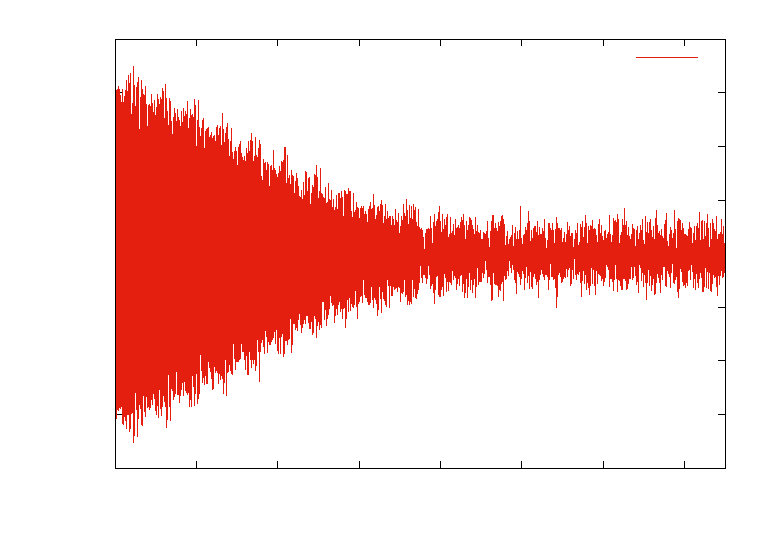
\includegraphics{plots/PulsandcollectValesignal}}%
    \gplfronttext
  \end{picture}%
\endgroup

    \caption[Example signal for a pulse and collect signal made by the B$_1$ coil.]{Example signal for a pulse and collect signal made by the B$_1$ coil.
    The example signal is taken from a FID signal.}
    \label{fig: PulsandcollectValesignal}
\end{figure}

Due to the fact that the B$_1$ coil is a tuned LCR circuit a resonance frequency exists, which can be calculated by the following formula:
\begin{align}
    \omega_{calc} = \frac{1}{\sqrt{L \cdot C}} \ .
    \label{eq: larmorcalc}
\end{align}
In order to analyse the B$_1$ coil the resonance frequency, depending on the capacity, is measured.
Therefore the B$_1$ coil transmits a signal.
Due to this signal the response of the coil can be measured.
This signal is then fourier transformed and the resonance frequency can be deduced from the frequency domain (maximum in the frequency domain).
This procedure is repeated automatically by the computer programm \textit{Prospa} for different capacities.
By changing the capacity we can examine the best capacity in dependence of the larmor frequency.
Figure \ref{fig: Coilanalyse} shows the measured and theoretically calculated resonance frequency (equation \eqref{eq: larmorcalc}; $L = \SI{0.417}{\henry}$) in dependence of the capacity.
The horizontal line represents the larmor frequency of \SI{1841.4}{\hertz} for hydrogen in Germany in July 2020.
To gain this value the vertical component of the earths magnetic field (\SI{43248.8}{\nano \tesla} \cite{magnetfeld}) is multiplied by the gyromagnetic ratio $\SI{42.577}{\frac{\mega \hertz}{\tesla}}$ \cite{magnetfeld}.
The vertical line represents the correct capacity we should use for our measurement, due to the resonance frequency of the larmor frequency.
In this case the correct capacity is \SI{13.8}{\nano \farad}.
Corresponding to the calculated resonance frequency the correct capacity would be \SI{17.9}{\nano \farad}.
It is not deniable that the measured curve is not parallel to the measured resonance frequency.
This probably has its cause in the not fixed inductance $L$.
Due to heating of the coil $L$ might change a little by increasing capacity and thus the calculated curve does not fit to the measured one.
Another reason for the different calculated curve is that we used real coils and those have parasite resistances and also built-in capacities.
This built-in capacity is not taken into account in the formula \eqref{eq: larmorcalc} and therefore the calculated curve might be not correct.
Since the calculated curve does not fit to the measured one, the calculated value for the capacity is not taken into account.

\begin{figure}[H]
    \centering
    % GNUPLOT: LaTeX picture with Postscript
\begingroup
  % Encoding inside the plot.  In the header of your document, this encoding
  % should to defined, e.g., by using
  % \usepackage[cp1252,<other encodings>]{inputenc}
  \inputencoding{cp1252}%
  \makeatletter
  \providecommand\color[2][]{%
    \GenericError{(gnuplot) \space\space\space\@spaces}{%
      Package color not loaded in conjunction with
      terminal option `colourtext'%
    }{See the gnuplot documentation for explanation.%
    }{Either use 'blacktext' in gnuplot or load the package
      color.sty in LaTeX.}%
    \renewcommand\color[2][]{}%
  }%
  \providecommand\includegraphics[2][]{%
    \GenericError{(gnuplot) \space\space\space\@spaces}{%
      Package graphicx or graphics not loaded%
    }{See the gnuplot documentation for explanation.%
    }{The gnuplot epslatex terminal needs graphicx.sty or graphics.sty.}%
    \renewcommand\includegraphics[2][]{}%
  }%
  \providecommand\rotatebox[2]{#2}%
  \@ifundefined{ifGPcolor}{%
    \newif\ifGPcolor
    \GPcolorfalse
  }{}%
  \@ifundefined{ifGPblacktext}{%
    \newif\ifGPblacktext
    \GPblacktexttrue
  }{}%
  % define a \g@addto@macro without @ in the name:
  \let\gplgaddtomacro\g@addto@macro
  % define empty templates for all commands taking text:
  \gdef\gplbacktext{}%
  \gdef\gplfronttext{}%
  \makeatother
  \ifGPblacktext
    % no textcolor at all
    \def\colorrgb#1{}%
    \def\colorgray#1{}%
  \else
    % gray or color?
    \ifGPcolor
      \def\colorrgb#1{\color[rgb]{#1}}%
      \def\colorgray#1{\color[gray]{#1}}%
      \expandafter\def\csname LTw\endcsname{\color{white}}%
      \expandafter\def\csname LTb\endcsname{\color{black}}%
      \expandafter\def\csname LTa\endcsname{\color{black}}%
      \expandafter\def\csname LT0\endcsname{\color[rgb]{1,0,0}}%
      \expandafter\def\csname LT1\endcsname{\color[rgb]{0,1,0}}%
      \expandafter\def\csname LT2\endcsname{\color[rgb]{0,0,1}}%
      \expandafter\def\csname LT3\endcsname{\color[rgb]{1,0,1}}%
      \expandafter\def\csname LT4\endcsname{\color[rgb]{0,1,1}}%
      \expandafter\def\csname LT5\endcsname{\color[rgb]{1,1,0}}%
      \expandafter\def\csname LT6\endcsname{\color[rgb]{0,0,0}}%
      \expandafter\def\csname LT7\endcsname{\color[rgb]{1,0.3,0}}%
      \expandafter\def\csname LT8\endcsname{\color[rgb]{0.5,0.5,0.5}}%
    \else
      % gray
      \def\colorrgb#1{\color{black}}%
      \def\colorgray#1{\color[gray]{#1}}%
      \expandafter\def\csname LTw\endcsname{\color{white}}%
      \expandafter\def\csname LTb\endcsname{\color{black}}%
      \expandafter\def\csname LTa\endcsname{\color{black}}%
      \expandafter\def\csname LT0\endcsname{\color{black}}%
      \expandafter\def\csname LT1\endcsname{\color{black}}%
      \expandafter\def\csname LT2\endcsname{\color{black}}%
      \expandafter\def\csname LT3\endcsname{\color{black}}%
      \expandafter\def\csname LT4\endcsname{\color{black}}%
      \expandafter\def\csname LT5\endcsname{\color{black}}%
      \expandafter\def\csname LT6\endcsname{\color{black}}%
      \expandafter\def\csname LT7\endcsname{\color{black}}%
      \expandafter\def\csname LT8\endcsname{\color{black}}%
    \fi
  \fi
    \setlength{\unitlength}{0.0500bp}%
    \ifx\gptboxheight\undefined%
      \newlength{\gptboxheight}%
      \newlength{\gptboxwidth}%
      \newsavebox{\gptboxtext}%
    \fi%
    \setlength{\fboxrule}{0.5pt}%
    \setlength{\fboxsep}{1pt}%
\begin{picture}(7200.00,5040.00)%
    \gplgaddtomacro\gplbacktext{%
      \csname LTb\endcsname%%
      \put(946,704){\makebox(0,0)[r]{\strut{}$1500$}}%
      \put(946,1527){\makebox(0,0)[r]{\strut{}$2000$}}%
      \put(946,2350){\makebox(0,0)[r]{\strut{}$2500$}}%
      \put(946,3173){\makebox(0,0)[r]{\strut{}$3000$}}%
      \put(946,3996){\makebox(0,0)[r]{\strut{}$3500$}}%
      \put(946,4819){\makebox(0,0)[r]{\strut{}$4000$}}%
      \put(1794,484){\makebox(0,0){\strut{}$6$}}%
      \put(2688,484){\makebox(0,0){\strut{}$8$}}%
      \put(3583,484){\makebox(0,0){\strut{}$10$}}%
      \put(4477,484){\makebox(0,0){\strut{}$12$}}%
      \put(5372,484){\makebox(0,0){\strut{}$14$}}%
      \put(6266,484){\makebox(0,0){\strut{}$16$}}%
    }%
    \gplgaddtomacro\gplfronttext{%
      \csname LTb\endcsname%%
      \put(209,2761){\rotatebox{-270}{\makebox(0,0){\strut{}Frequency $\si{\hertz}$}}}%
      \put(3940,154){\makebox(0,0){\strut{}Capacity in $\si{\nano \farad}$}}%
      \csname LTb\endcsname%%
      \put(5816,4646){\makebox(0,0)[r]{\strut{}measured resonance frequency}}%
      \csname LTb\endcsname%%
      \put(5816,4426){\makebox(0,0)[r]{\strut{}calculated resonance frequency}}%
    }%
    \gplbacktext
    \put(0,0){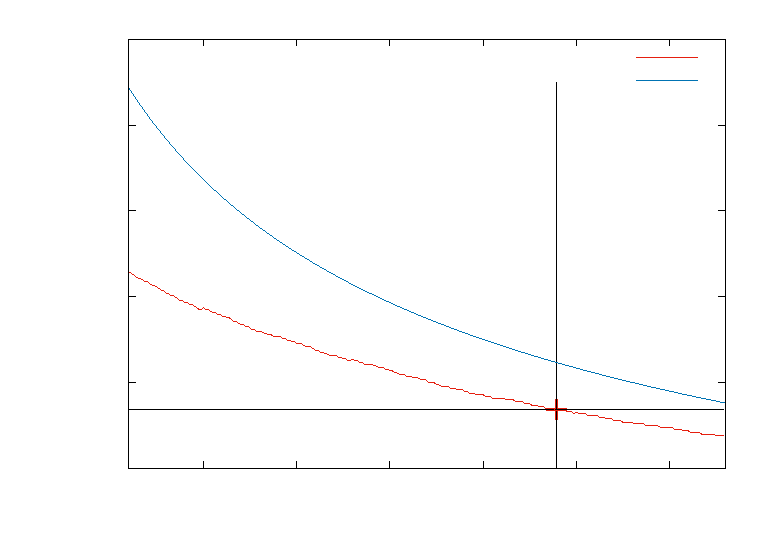
\includegraphics{plots/Coilanalyse}}%
    \gplfronttext
  \end{picture}%
\endgroup

    \caption[This figure shows the measured and calculated resonance frequencies for different capacities.]{This figure shows the measured and calculated resonance frequencies for different capacities.
    The marked cross represents the larmor frequency of \SI{1841.4}{\hertz} for hydrogen in Germany in July 2020.}
    \label{fig: Coilanalyse}
\end{figure}